\documentclass[a4paper, 12pt]{article}%тип документа

%отступы
\usepackage[left=2cm,right=2cm,top=2cm,bottom=3cm,bindingoffset=0cm]{geometry}

%Русский язык
\usepackage[T2A]{fontenc} %кодировка
\usepackage[utf8]{inputenc} %кодировка исходного кода
\usepackage[english,russian]{babel} %локализация и переносы

%Вставка картинок
\usepackage{wrapfig}
\usepackage{graphicx}
\graphicspath{{pictures/}}
\DeclareGraphicsExtensions{.pdf,.png,.jpg}

%оглавление
\usepackage{titlesec}
\titlespacing{\chapter}{0pt}{-30pt}{12pt}
\titlespacing{\section}{\parindent}{5mm}{5mm}
\titlespacing{\subsection}{\parindent}{5mm}{5mm}
\usepackage{setspace}

%Графики
\usepackage{multirow}
\usepackage{pgfplots}
\pgfplotsset{compat=1.9}

%Математика
\usepackage{amsmath, amsfonts, amssymb, amsthm, mathtools}

%Заголовок
\author{Валеев Рауф Раушанович \\
группа 825}
\title{\textbf{Работа 5.6\\
Измерение $\beta$-спектров с помощью сцинтилляционного пластикового детектора}}
\newtheorem{task}{Задача}
\begin{document}
\maketitle
\newpage
\paragraph*{Цель работы:} Измерить $\gamma$ и $\beta$-спектры $^{137}Cs$, $^{90}Sr$, $^{36}Cl$, $^{60}Co$ и $^{22}Na$. И с помощью них измерить граничные энергии электронов и позитронов, энергию края комптоновского рассеяния.
\section*{Теория}
\subsection*{Принцип $\beta$-распада}
Для спектрометрии гамма-излучения используется обычно неорганический кристалл $NaI(Tl)$. На рис. 1 в качестве примера показан спектр $^{60}Co$. Следует подчеркнуть, что в подавляющем большинстве случаев искусственные источники гамма-излучения являются бета-источниками, в которых после бета-распада образуется дочернее ядро в возбужденном состоянии. В данном случае мы имеем дело с бета-переходом из $^{60}Co$ в ядро $^{60}Ni$, как это показано на рисунке. Время жизни этого гамма-источника определяется периодом полураспада $^{60}Co$, равного 5,2 года, а время гамма-переходов при снятии возбуждения в ядре $^{60}Ni$ очень мало ($\approx 10^{-10}$ с).

\begin{figure}[h]
\begin{center}
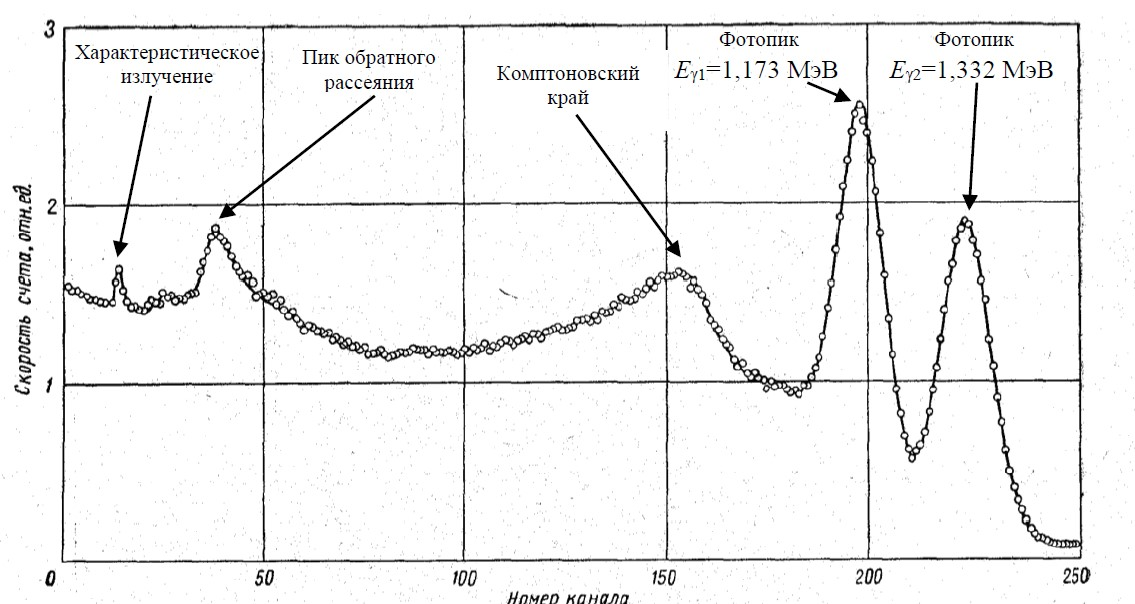
\includegraphics[width = \textwidth]{1.jpg}
\caption{Гамма-спектр радиоактивного источника $^{60}Co$, полученный при ре-гистрации излучения сцинтилляционным гамма-спектрометром с кристаллом NaI(Tl). В нижней части рисунка показана схема распада этого ядра.}
\end{center}
\end{figure}

На данном графике приведен $\gamma$-спектр $^{60}Co$ по которому мы в дальнейшем будем понимать для других элементов, что мы меряем.
\newpage
\begin{figure}[h]
\begin{center}
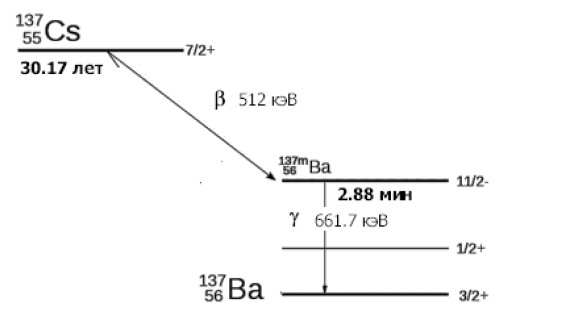
\includegraphics[width = 0.45\textwidth]{2.jpg}
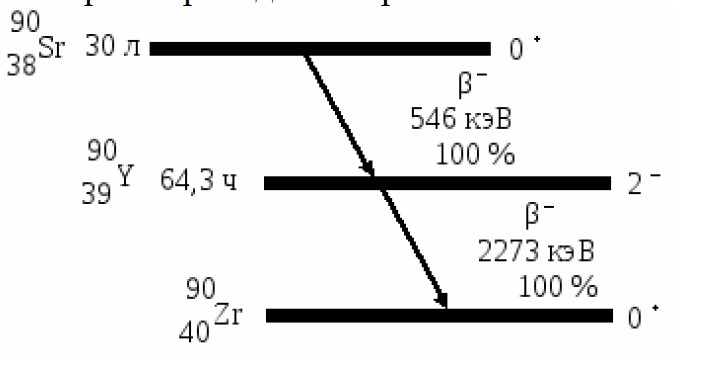
\includegraphics[width = 0.45\textwidth]{3.jpg}
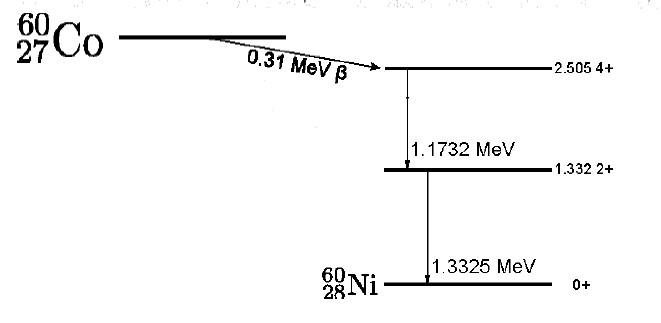
\includegraphics[width = 0.45\textwidth]{4.jpg}
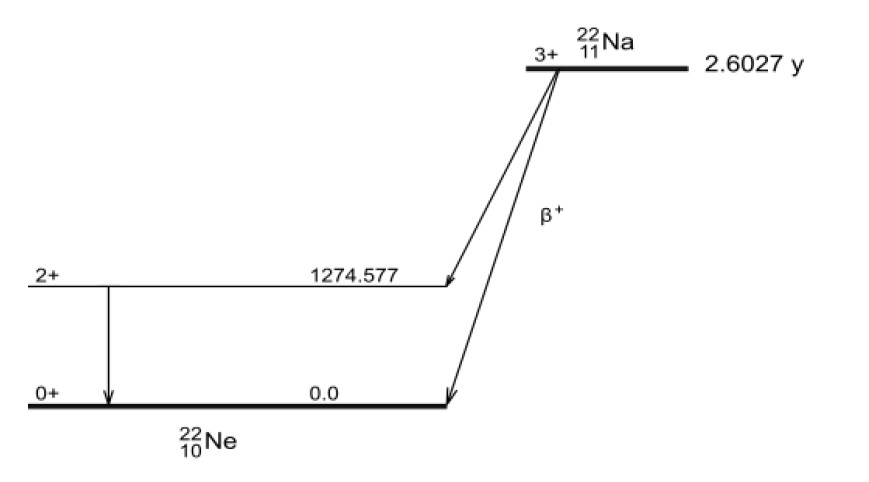
\includegraphics[width = 0.45\textwidth]{5.jpg}
\caption{Схемы распада различных элементов}
\end{center}
\end{figure}

\section*{Схема установки}
\begin{figure}[h]
\begin{center}
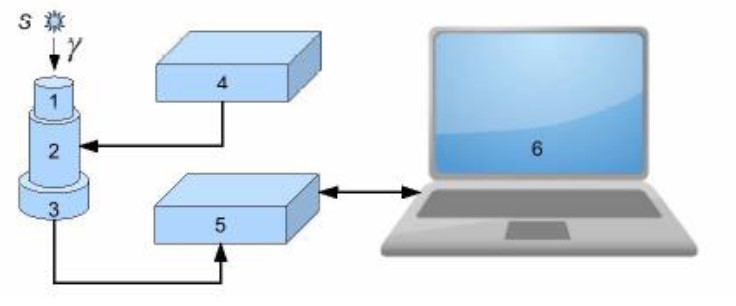
\includegraphics[width = 0.7\textwidth]{6.jpg}
\caption{Принципиальная блок-схема установки}
\end{center}
\end{figure}
На этом рисунке: 1 – сцинтиллятор, 2 – ФЭУ, 3 – предусилитель импульсов, 4 – высоковольтный блок питания для ФЭУ, 5 – блок преобразования
аналоговых импульсов с ФЭУ в цифровой код (АЦП), 6 – компьютер для
сбора данных, их обработки и хранения.
\section*{Метод наименьших квадратов для параболы}
В дальнейшем нам много где понадобится метод наименьших квадратов для параболы, поэтому здесь мы выведем формулу для определения пика параболы, чтобы использовать ее в дальнейшем.

Сама функция выглядит следующим образом:
\[f(x) = ax^2 + bx + c\]

Приведем сам метод:
\[F(a, b, c) = \sum\limits_{i = 1}^{n} \left(y_i - f(x_i)\right)^2\]
Найдем минимум этой функции:
\[\frac{\partial F}{\partial a} = \sum\limits_{i = 1}^n  -2(y_i - ax_i^2 - bx_i - c)(-x_i^2)\]
\[\frac{\partial F}{\partial a} = \sum\limits_{i = 1}^n  -2(y_i - ax_i^2 - bx_i - c)(-x_i)\]
\[\frac{\partial F}{\partial a} = \sum\limits_{i = 1}^n  -2(y_i - ax_i^2 - bx_i - c)(-1)\]

Теперь решим систему частных производных равных 0 $\Rightarrow$
\[\begin{cases}
\sum\limits_{i = 1}^n x_i^2 y_i = a \sum\limits_{i = 1}^n x_i^4 + b\sum\limits_{i = 1}^n x_i^3 + c \sum\limits_{i = 1}^n x_i^2\\
\sum\limits_{i = 1}^n x_i y_i = a \sum\limits_{i = 1}^n x_i^3 + b\sum\limits_{i = 1}^n x_i^2 + c \sum\limits_{i = 1}^n x_i\\
\sum\limits_{i = 1}^n y_i = a \sum\limits_{i = 1}^n x_i^2 + b\sum\limits_{i = 1}^n x_i + c n
\end{cases}\]

Решением будет
\[a = \frac{\left<y_i x_i^2\right> - b \left<x_i^3\right> - c \left<x_i^2\right>}{\left<x_i^4\right>}\]
\[b = \frac{\left<y_ix_i\right>\left<x_i^4\right> - \left<y_ix_i^2\right>\left<x_i^3\right> + c\left(\left<x_i^2\right>\left<x_i^3\right> - \left<x_i\right>\left<x_i^4\right>\right)}{\left<x_i^2\right> \left<x_i^4\right> - \left<x_i^3\right>^2}\]
\[c = \frac{\left<y_i x_i^2\right>^2 \left<x_i^2\right>^2 - \left<x_i^4\right> \left<x_i^3\right> \left<x_i^2\right> \left<y_ix_i\right> + \left<x_i^4\right>^2\left<y_i x_i\right>\left<x_i\right> + \left<x_i^4\right>\left<x_i^3\right>^2 \left<y_i\right> - \left<x_i^2 y_i\right>\left<x_i^4\right>\left<x_i^2\right>\left<y_i\right>} {\left<x_i^4\right>\left<x_i^3\right>^2 - \left<y_i x_i^2\right>\left<x_i^4\right>\left<x_i^2\right> + \left<x_iy_i^2\right>\left<x_i^2\right>^3 - 2\left<x_i^4\right>\left<x_i^3\right>\left<x_i^2\right>\left<x_i\right> + \left<x_i^4\right>^2\left<x_i\right>^6}\]

Далее находим пик как
\[x_c = \frac{-b}{2a}\]
Погрешность будет равна
\[\sigma_{x_c} = x_c\sqrt{\left(\frac{\sigma_b}{b}\right)^2 + \left(\frac{\sigma_a}{a}\right)^2}\]
\section*{Определение точки пересечения двух прямых}
В некоторых опытах нам может понадобится по графику определить переломную точку. Это мы можем сделать построив две прямые по мнк по формуле для прямой: $y = kx + b$, тогда из мнк 
\[k = \frac{\left<xy\right>  - \left<x\right>\left<y\right>}{\left<x^2\right> - \left<x\right>^2}\]
\[\sigma_k = \sqrt{\frac{1}{n-1} \left(\frac{\left<y^2\right>}{\left<y\right>^2} - k^2\right)}\]
\[b = (\left<y\right> - k\left<x\right>)\]
\[\sigma_b =  \sigma_k\sqrt{\left<x^2\right>}\]

Тогда после аппроксимации у нас будут две прямые: $f_1(x) = k_1 x + b_1$,$f_2(x) = k_2 x + b_2$. 

Найдем их точку пересечения. Будем все делать только для $x$, поскольку нас интересует только номер канала
\[x = \frac{b_2 - b_1}{k_1 - b_2}\]
Из этого следует, что 
\[\sigma_x = \sqrt{\left( \frac{\sigma_{b_1}}{b_1}\right)^2 + \left( \frac{\sigma_{b_2}}{b_2}\right)^2 + \left( \frac{\sigma_{k_1}}{k_1}\right)^2 + \left( \frac{\sigma_{k_2}}{k_2}\right)^2}\]
\section*{Ход работы}
Для начала замерим фон, для этого удалим из свинцового блока все образцы, после чего замерим спектр.

\begin{figure}[h]
\begin{center}
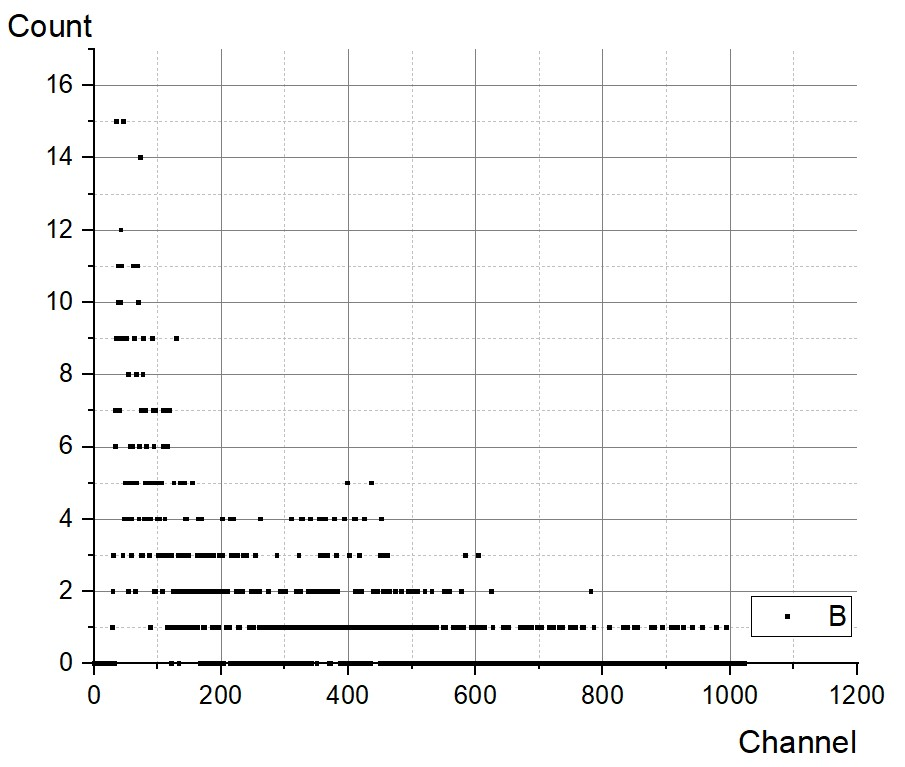
\includegraphics[width = 0.6\textwidth]{7.jpg}
\caption{Спектр фонового шума}
\end{center}
\end{figure}

Как мы увидим в дальнейшем, средняя амплитуда спектра фонового шума отличается на 3 порядка от амплитуды пиков, которые мы меряем, из чего следует вывод, что наша установка хорошо изолирована от внешних частиц.
\newpage
\subsection*{Cs$^{137}$}
Построим график распределения частиц и по нему проведем нормировку каналов по энергии. При распаде Cs$^137$ преимущественно возникают электроны с граничной энергией $0,512$ МэВ. Кроме того возникают электроны внутренней конверсии с энергией $0,624$ МэВ. Однако комптоновский край от гамма-квантов накладывается на пик электронов, поэтому мы нормируем только по энергии внутренней конверсии.

Для сцинтилляционного детектора номер канала пропорционален энергии электронов. Зная номер канала $N_k$ и энергию $E_k$ конверсионных электронов, постройте линейный калибровочный график зависимости номера канала $N_i$ от энергии $E_i$: $N_i = a E_i$. 

По графику мы можем определить, что пик находится в $157,2 \pm 0,2$ канале. Пик определяем по параболе, найдем его так, как было расписано в начале работы.

\begin{figure}[h]
\begin{center}
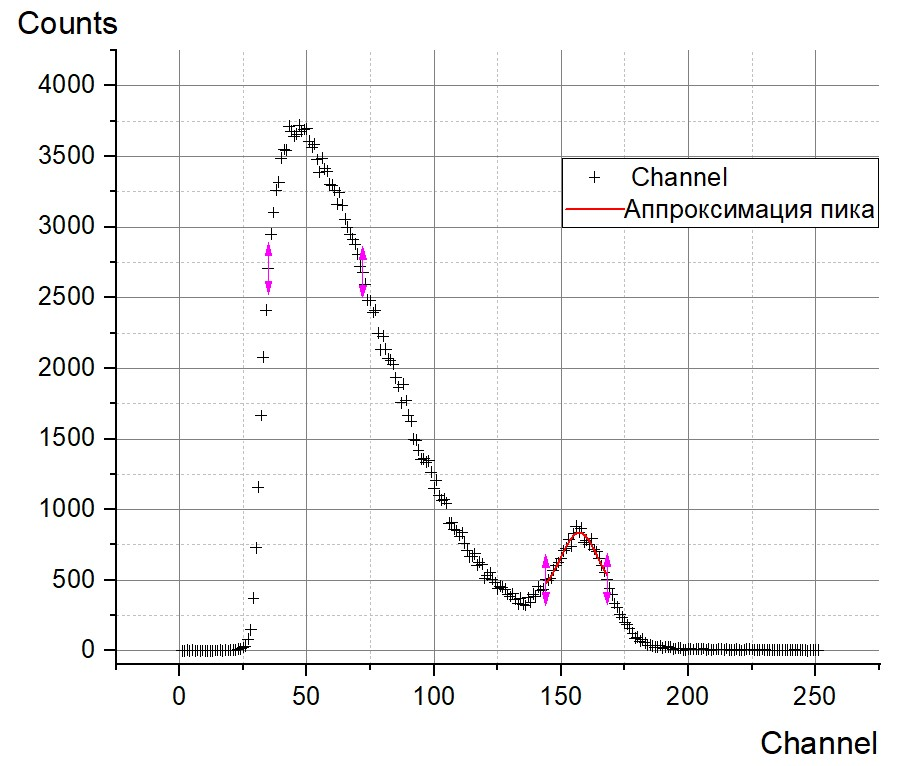
\includegraphics[width = \textwidth]{8.jpg}
\caption{Cs$^{137}$}
\end{center}
\end{figure}

Далее проводим нормировку:
\[a = \frac{N_k}{E_k} = 251,9 \pm 0,3 \frac{\text{канал}}{\text{МэВ}}\]
\newpage
\subsection*{Cs$^{137}$ с монетой}

Сделаем то же, что мы делали в предыдущем пункте, только найдем пик от гамма квантов

\begin{figure}[h]
\begin{center}
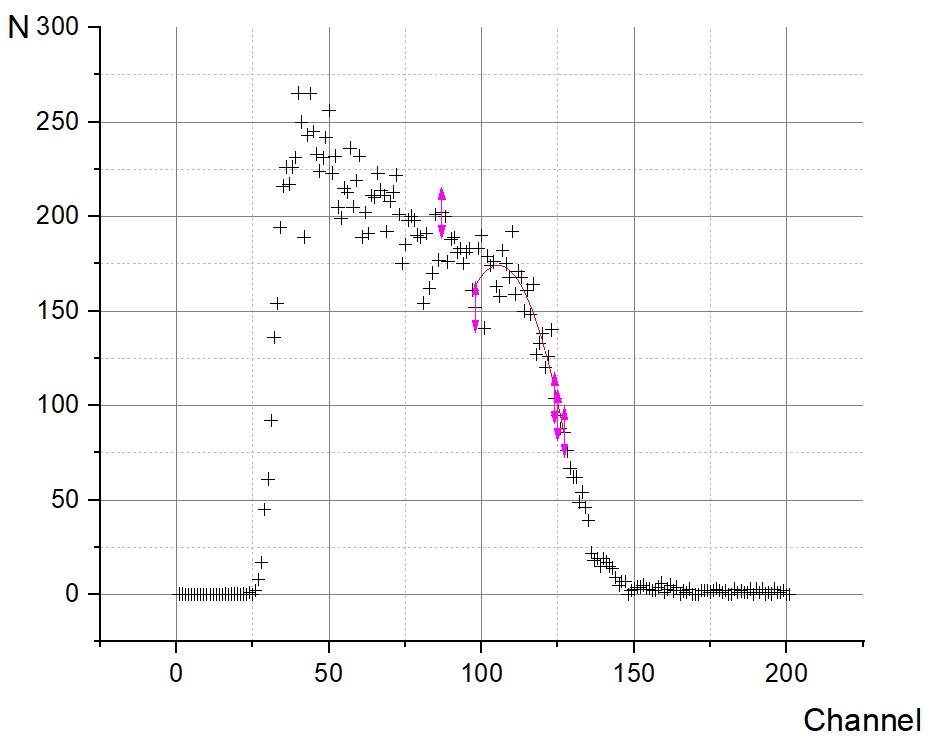
\includegraphics[width = \textwidth]{9.jpg}
\caption{Cs$^{137}$ с монетой}
\end{center}
\end{figure}
Пик в точке $168 \pm 1$, значит 
\[E_{\gamma} = \frac{a}{N} = 0,666 \pm 0,01 \text{МэВ}\]
Погрешность находим по формуле
\[\sigma_E = \sqrt{\frac{\sigma_a^2}{a^2} + \frac{\sigma_N^2}{N^2}}\]

Что в пределах погрешности совпадает с реальным значением $0,664$ МэВ.
\newpage
\subsection*{Cs$^{137}$ максимальная энергия электронов}
Найдем максимальную энергию электронов по разности графиков для цезия и цезия с монетой.

\begin{figure}[h]
\begin{center}
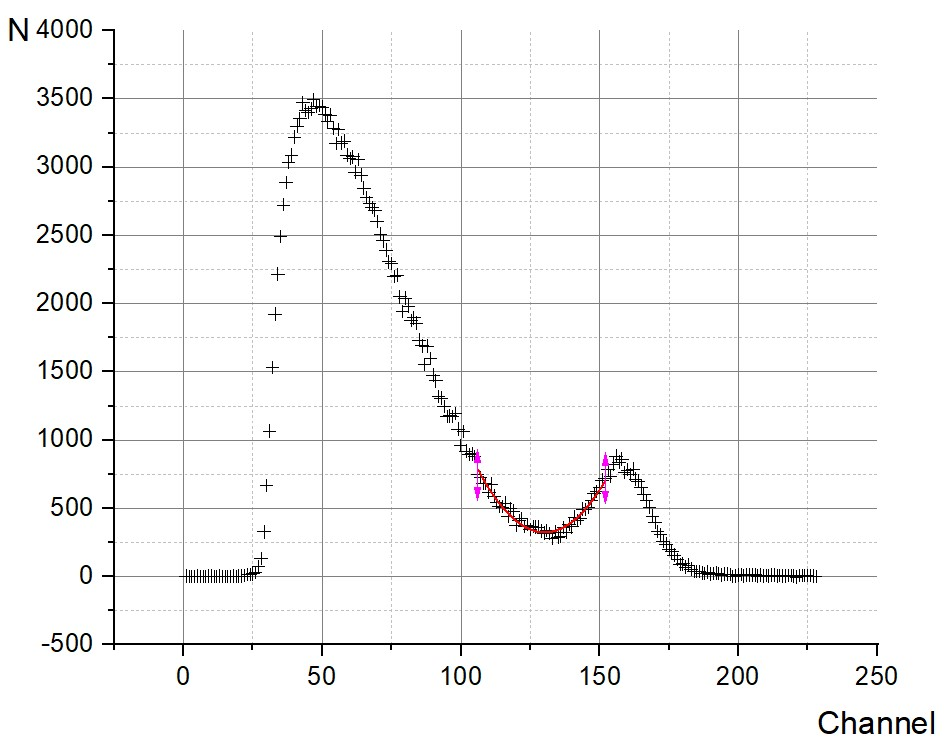
\includegraphics[width = \textwidth]{10.jpg}
\caption{Разность графиков для Cs$^{137}$}
\end{center}
\end{figure}

Пик в канале $131,2\pm 0,6$. Значит
\[E_{max} = 0,51 \pm 0,01 \text{МэВ}\]
Что в пределах погрешности совпадает с теоретической оценкой 
\[E_t = 0,512 \text{МэВ}\]
\newpage
\subsection*{Sr$^{90}$}
Сделаем то же, что и в предыдущих пунктах, только будем искать энергию из точек перегиба, как написано в теории.

В итоге мы получаем, что $x_1 = 127 \pm 3$, $x_2 = 533 \pm 5$.

\begin{figure}[h]
\begin{center}
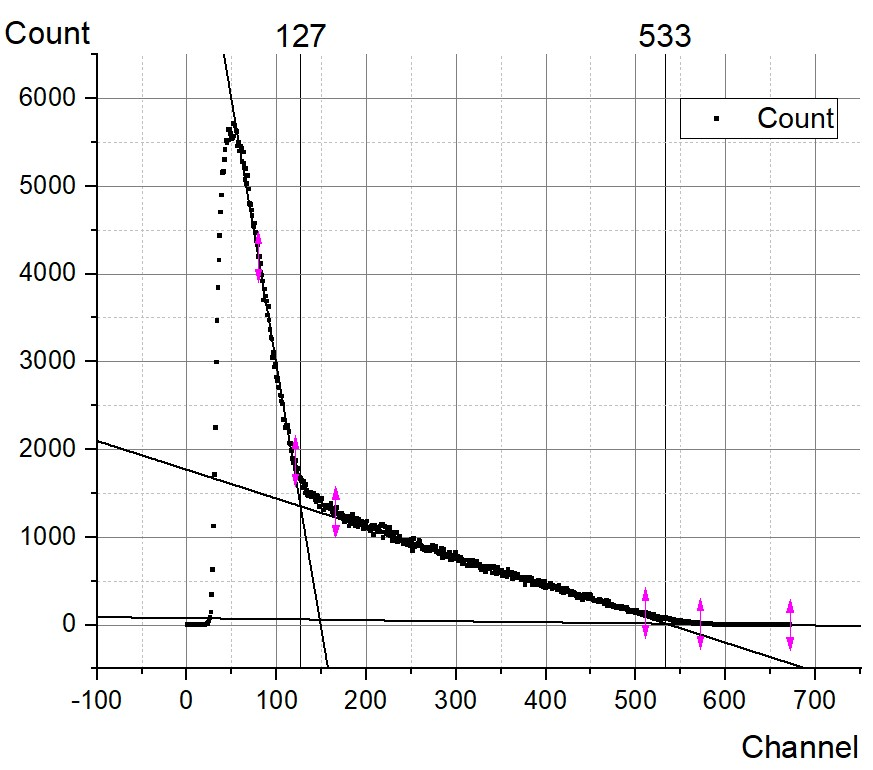
\includegraphics[width = \textwidth]{11.jpg}
\caption{Sr$^{90}$}
\end{center}
\end{figure}

По этим перегибам мы получаем, что \[E_1 = 0,51 \pm 0,02\text{МэВ}\] \[E_2 = 2,11 \pm 0,1\text{МэВ}\] Что с точностью до погрешностей совпадает с теоретическими данными $E_{1t} = 0,546$ МэВ, $E_2 = 2,273$ МэВ.
\newpage
\subsection*{Cl$^{36}$}
Здесь нам нужно найти предельную энергию электронов которую мы так же определим как точку пересечения двух прямых

\begin{figure}[h]
\begin{center}
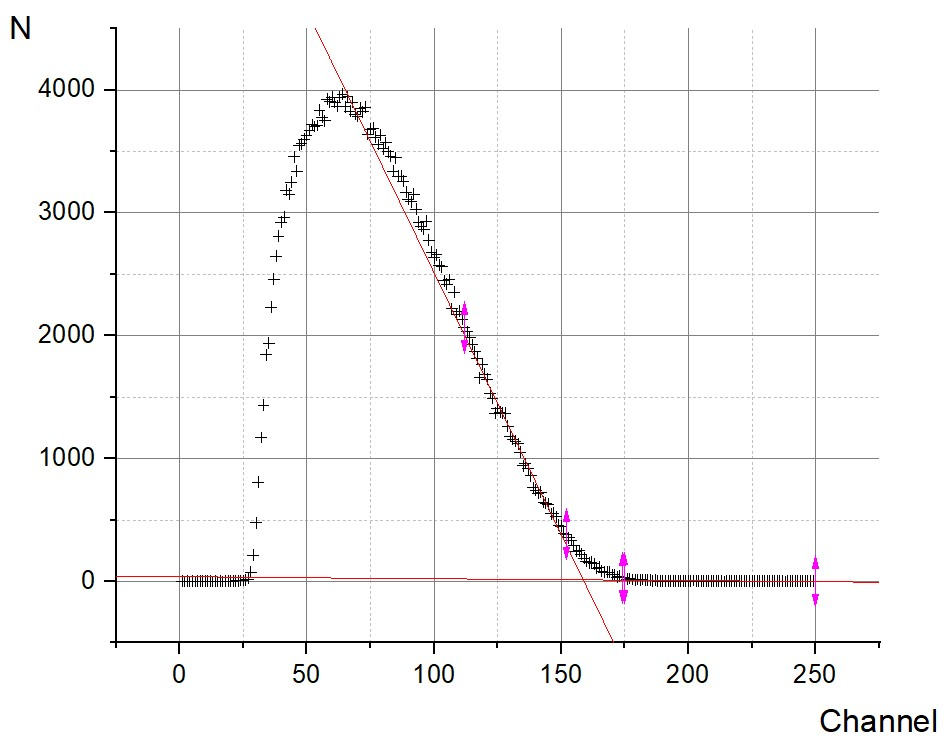
\includegraphics[width = \textwidth]{12.jpg}
\caption{Cl$^{36}$}
\end{center}
\end{figure}

В итоге получаем, что $x = 161 \pm 5$. А энергия получается
\[E = 0,64 \pm 0,03 \text{МэВ}\]

Что с точностью до 2 сигма совпадает с теоретическим значением
\[E_t = 0,714 \text{МэВ}\]
\newpage
\subsection*{Co$^{60}$}
Найдем граничные энергии для двух групп электронов 
\begin{figure}[h]
\begin{center}
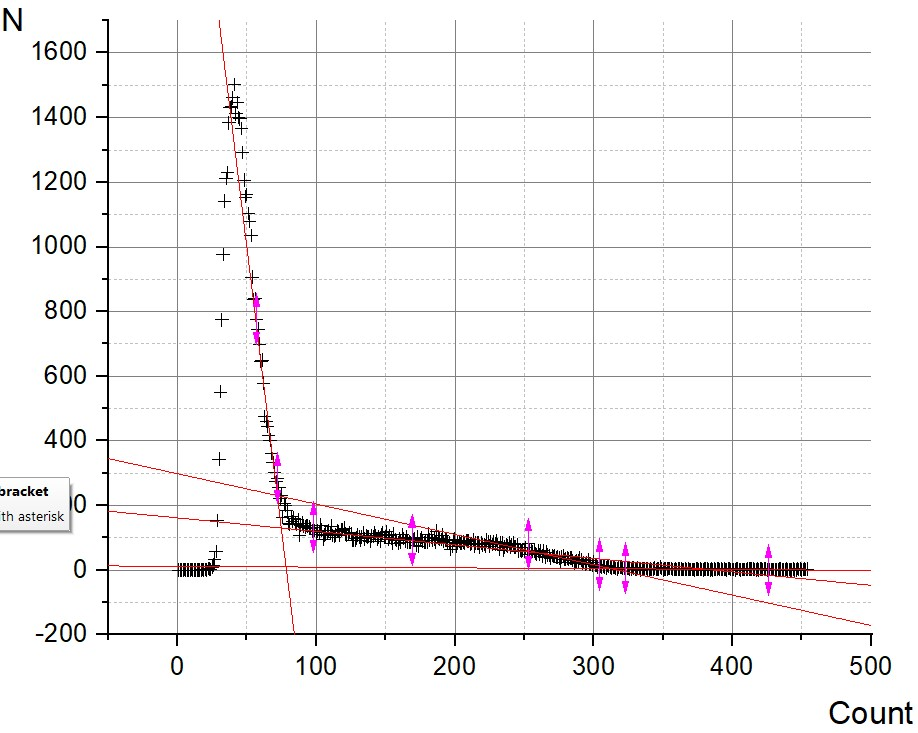
\includegraphics[width = \textwidth]{13.jpg}
\caption{Co$^{60}$}
\end{center}
\end{figure}

Номера каналов найдем как точки пересечения двух прямых: $x_1 = 0,29 \pm 0,02$, $x_2 = 300 \pm 20$ значит
\[E_1 = 0,29 \pm 0,02 \text{МэВ}\]
\[E_2 = 1,2 \pm 0,1 \text{МэВ}\]

Что с точностью до погрешностей совпадает с теоретическими
\[E_{1t} = 0,314 \text{МэВ}\]
\[E_{2t} = 1,48 \text{МэВ}\]
\newpage
\subsection*{Co$^{60}$ с монетой}
Из данного графика найдем край комптоновского рассеяния

\begin{figure}[h]
\begin{center}
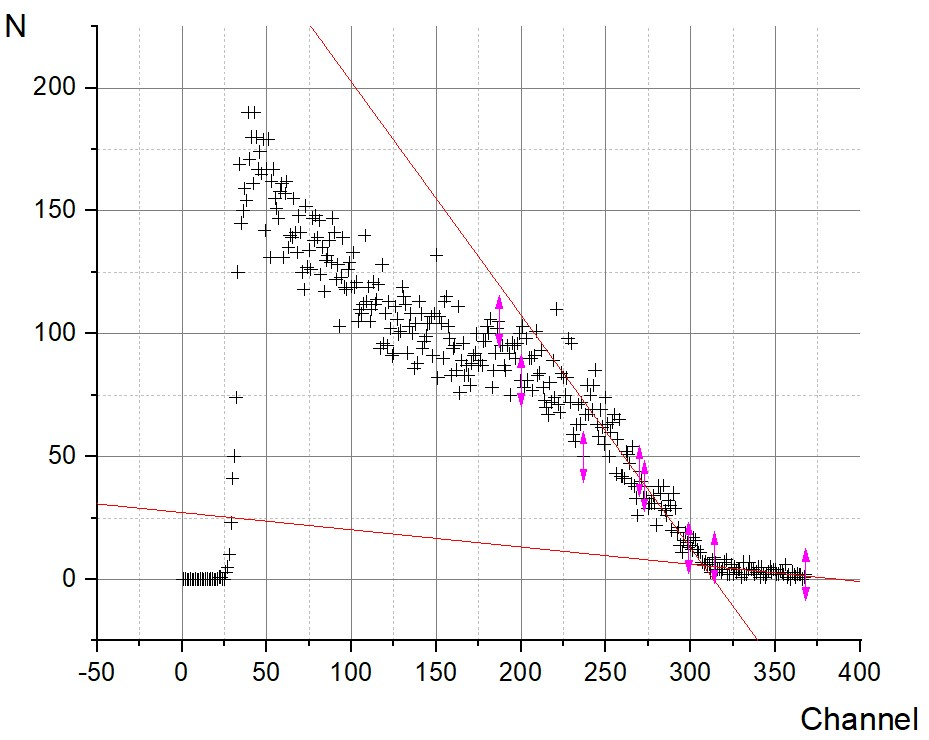
\includegraphics[width = \textwidth]{14.jpg}
\caption{Co$^{60}$}
\end{center}
\end{figure}

В итоге получаем $x = 310 \pm 30$.

Из этих данных мы получаем, что энергия равна 
\[E = 1,23 \pm 0,12 \text{МэВ}\]

Что с точностью до погрешности совпадает с теорией
\[E_t = 1,173 \text{МэВ}\]
\newpage
\subsection*{Граничная энергия позитронов при распаде Na$^{22}$}
Данную энергию мы получим из разности графиков с монетой и без.

\begin{figure}[h]
\begin{center}
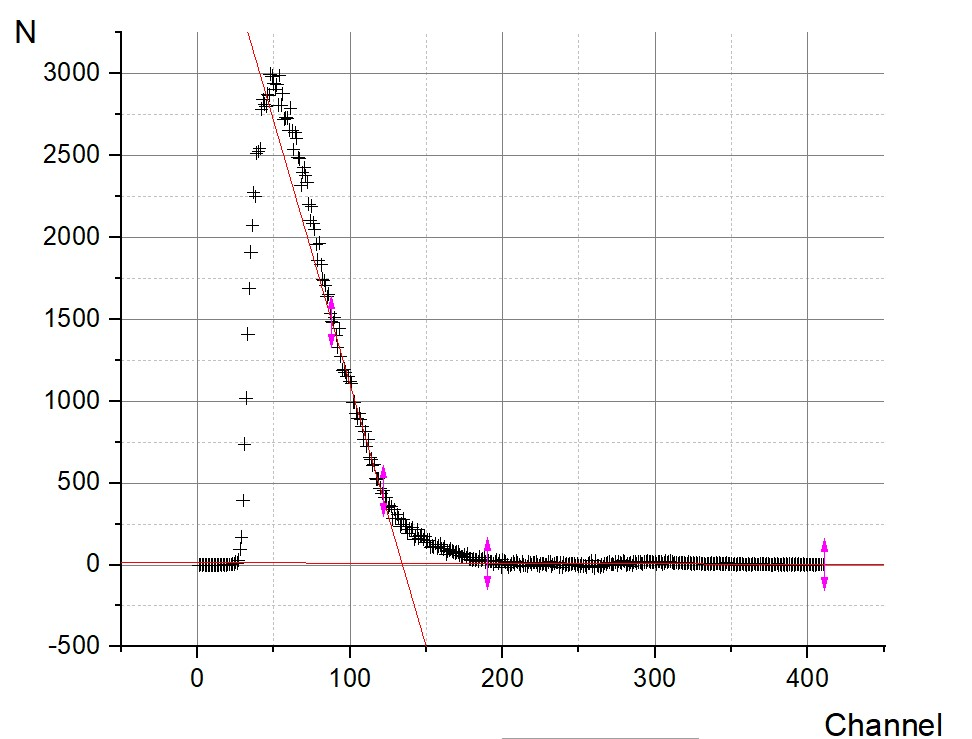
\includegraphics[width = \textwidth]{15.jpg}
\caption{Разность с монетой и без для Na$^{22}$}
\end{center}
\end{figure}

Из этого графика получаем, что $x = 134\pm 5$.Отсюда
\[E = 0,533 \pm 0,011 \text{МэВ}\]

Что совпадает с теоретическим значением, равным
\[E_t = 0,545 \text{МэВ}\]

\newpage

\subsection*{Край комптоновского рассеяния для двух гамма-квантов}

Эти энергии мы снимем для графика без монетки

\begin{figure}[h]
\begin{center}
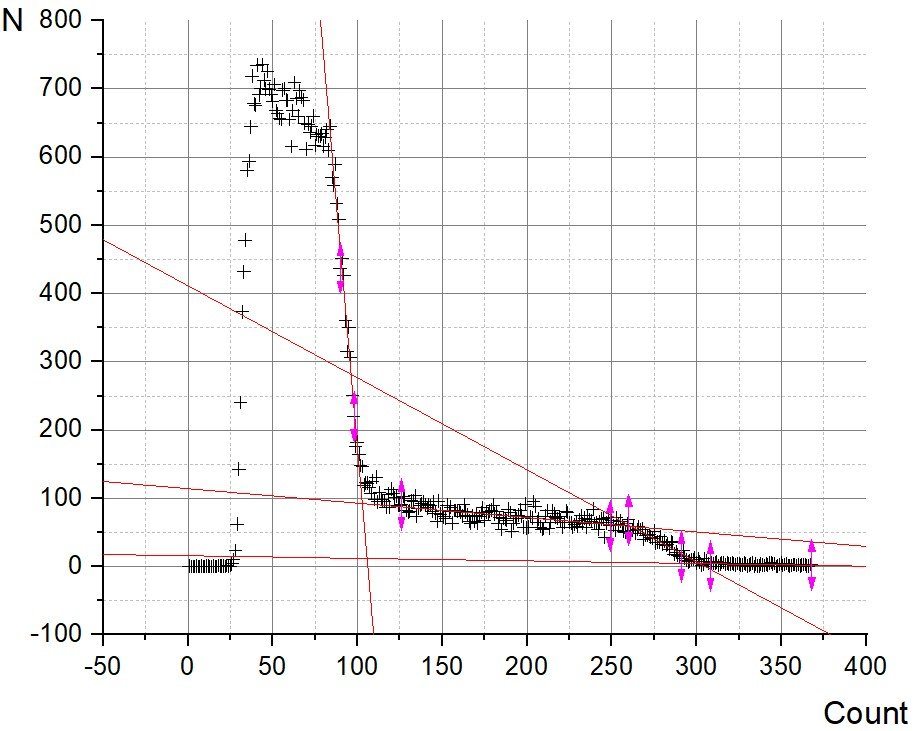
\includegraphics[width = \textwidth]{16.jpg}
\caption{Na$^{22}$ без монеты}
\end{center}
\end{figure}

В итоге мы получаем, что наши энергии равны
\[E_1 = 0,39 \pm 0,05 \text{МэВ}\]
\[E_2 = 1,23 \pm 0,04 \text{МэВ}\]

Что совпадает с теоретическими значениями.

\section*{Вывод}
Мы померяли некоторые граничные энергии для бетта-распадов различных частиц и убедились в правдивости теоретических подсчетов этих энергий.
\end{document}